\begin{frame}
\frametitle{The continuous beta spectrum}

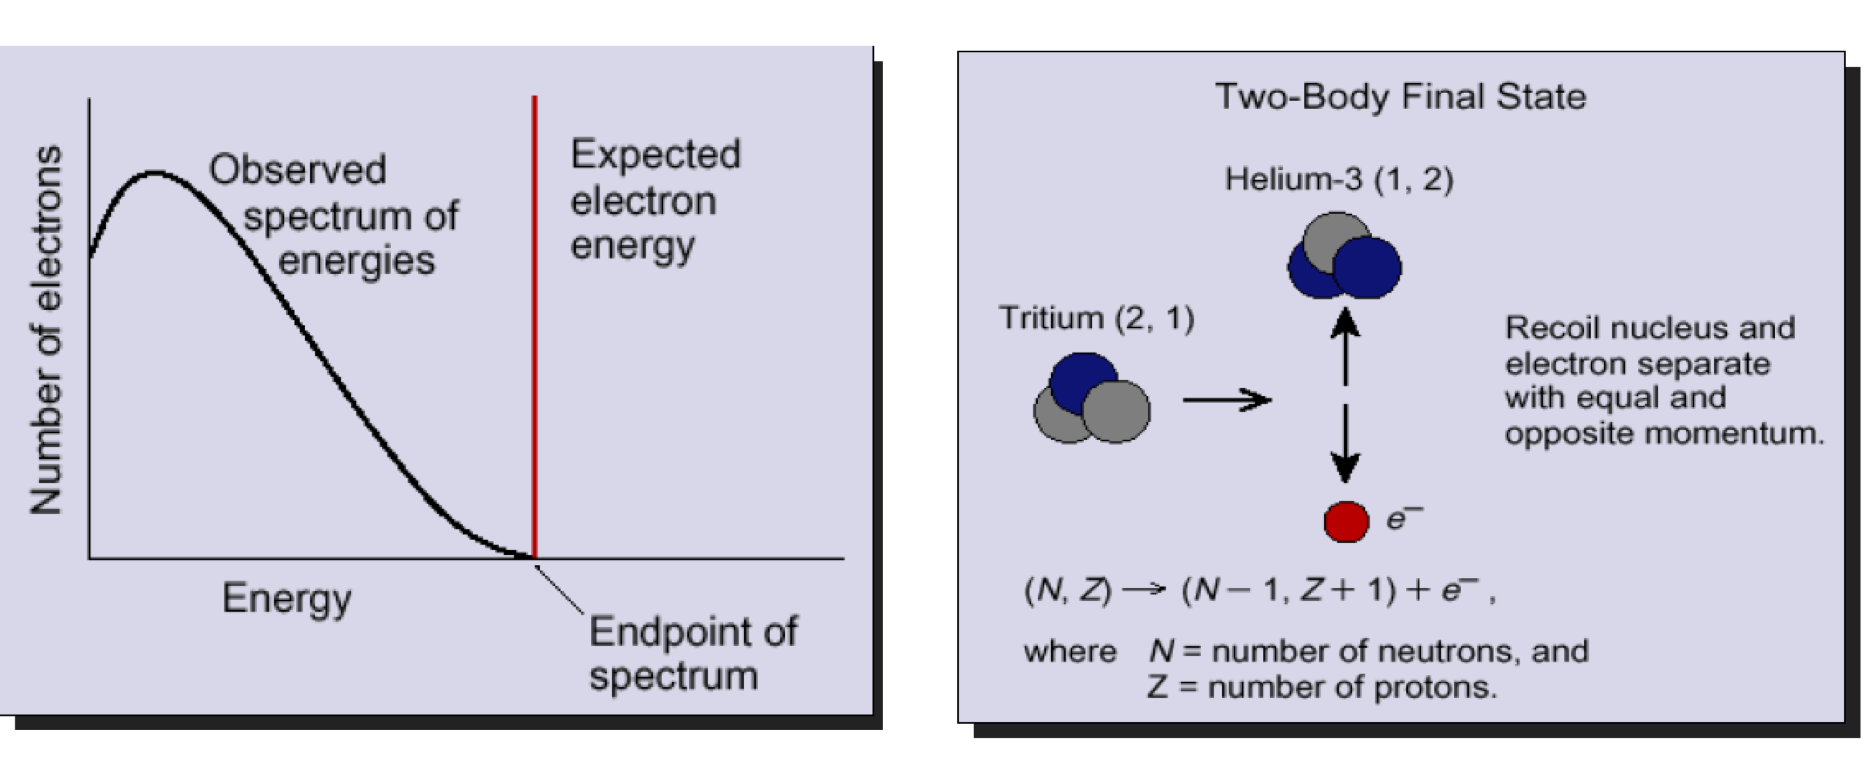
\includegraphics[scale=0.38]{pool/imgTalks/beta-ray.png}
 
\end{frame}


\begin{frame}
\frametitle{Liebe Radioaktive Damen und Herren}
\begin{columns}
 
\column{0.5\textwidth}
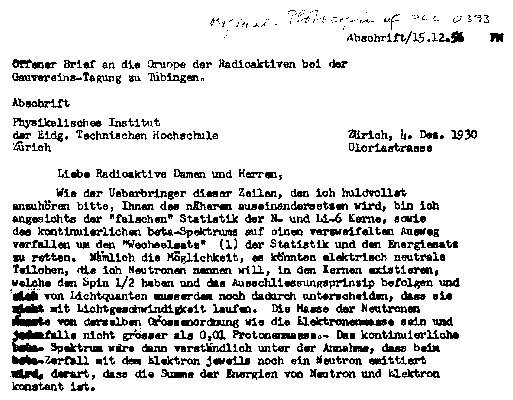
\includegraphics[scale=0.4]{liebe.png}
 
\column{0.2\textwidth}
\begin{block}{}
Dear Radioactive Ladies and Getlemen.

...because the continuous beta spectrum...I have hit upon a desperate remedy to save the law of conservation of energy.

\end{block}
\end{columns}
\end{frame}


\begin{frame}
\frametitle{Why so desperate?}

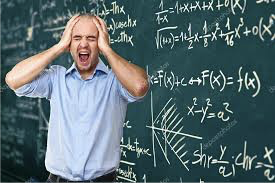
\includegraphics[scale=0.4]{desperate.png}
 

\begin{block}{}
Because conservation of energy-momentum means that physics does not depend on space-time translations. We believe that physics laws must be the same here than in Andromeda, and the same today than next or last year. Physicists, then, could not give up on energy conservation.

\end{block}

\end{frame}

\begin{frame}
\frametitle{Two and three body kinematics}

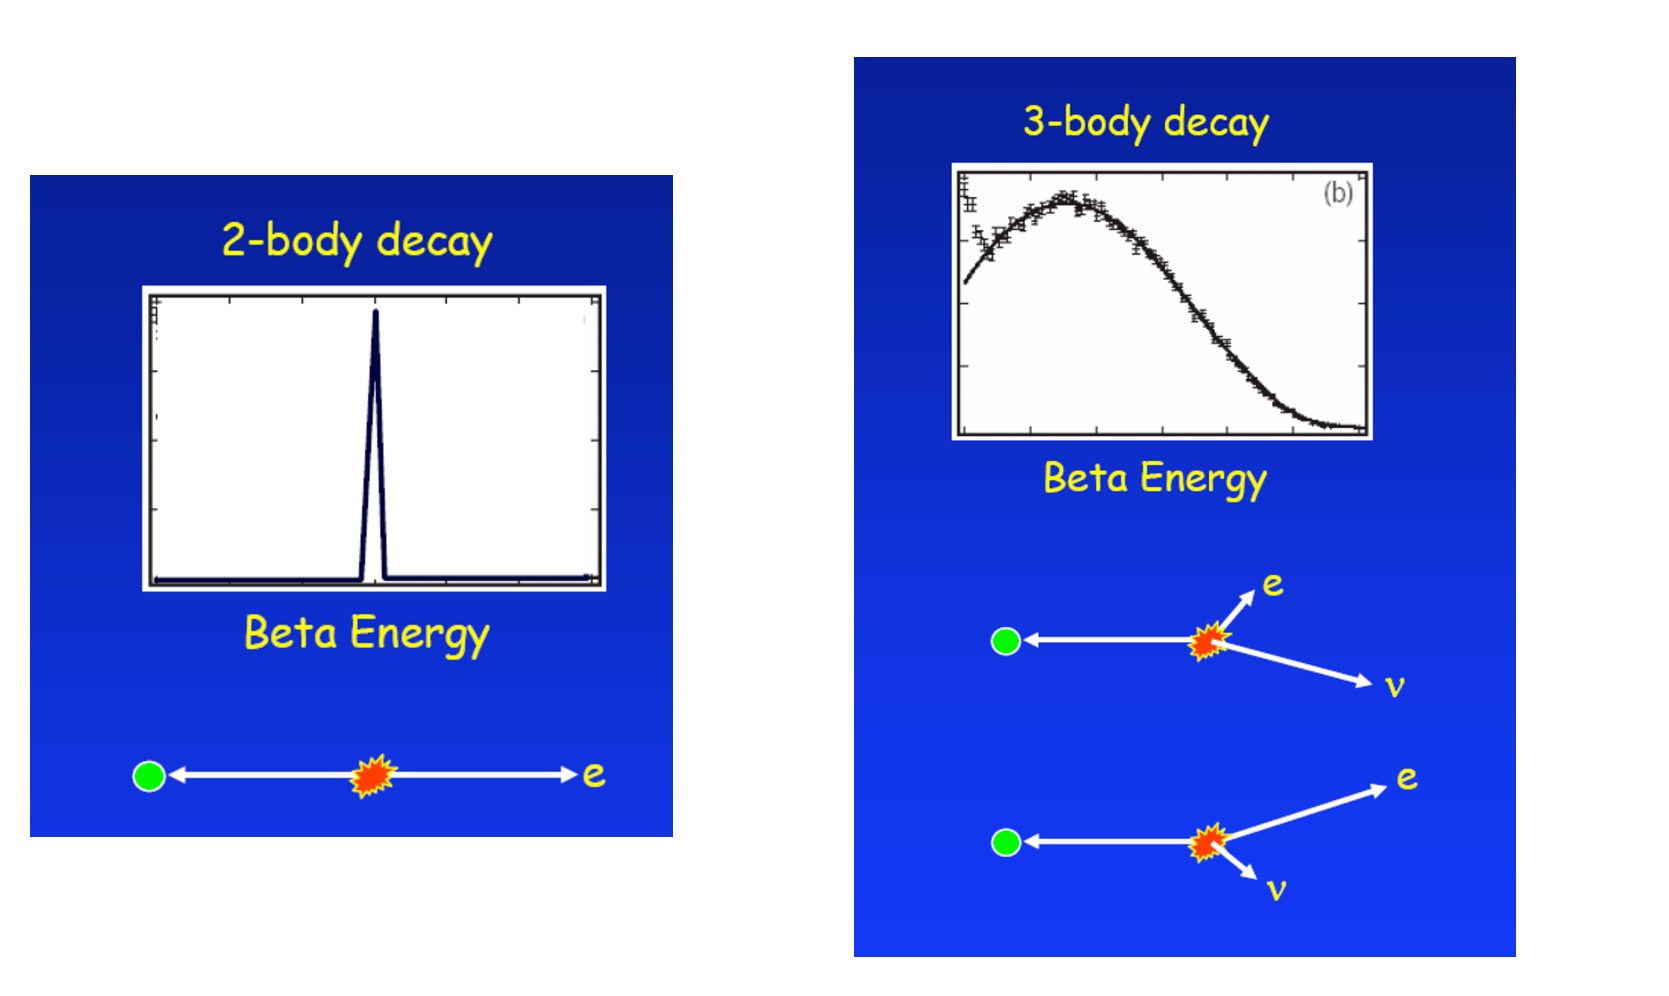
\includegraphics[scale=0.4]{kinematics.pdf}
 
\end{frame}

\begin{frame}
\frametitle{Pauli's neutrino}
\begin{columns}
\column{0.35\textwidth}
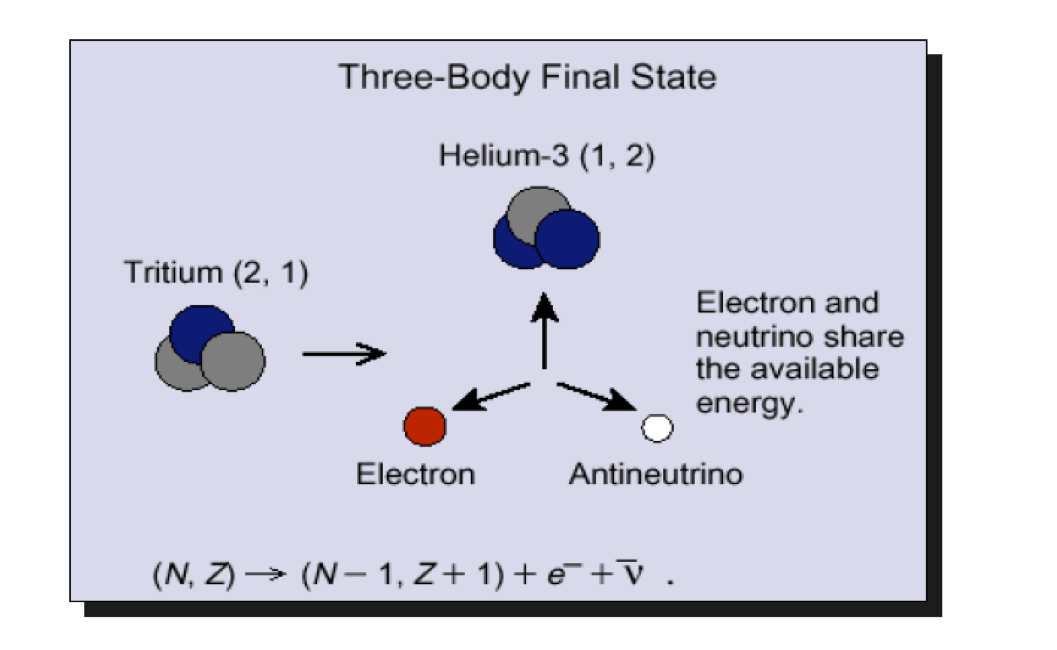
\includegraphics[scale=0.3]{pauli-neutrino.png}

\noindent Pauli in  1933 at the Solvay Congress: 

Regarding the properties of these neutral particles, the atomic weights
of the radioactive elements tell us first of all that their mass cannot exceed
much that of the electron.

 \column{0.50\textwidth}
 In order to distinguish them from the heavy
neutrons, Mr. Fermi proposed the name ``neutrino.'' {\bf It's possible that the
neutrinos' own mass might be equal to zero, so that they would have to
propagate with the speed of light, like the photons}. However, their penetrating power would exceed by far that of photons of the same energy. It
seems to me acceptable that the neutrinos have spin 1/2 and satisfy Fermi's 
statistics, although experiments do not give us any direct proof of this hypothesis. 
{\bf We know nothing about the interaction of the neutrinos with other material particles and with the photons".}
\end{columns}
\end{frame}

%\begin{frame}
%\frametitle{Pauli's neutrino}
%\begin{columns}
%\column{0.45\textwidth}
%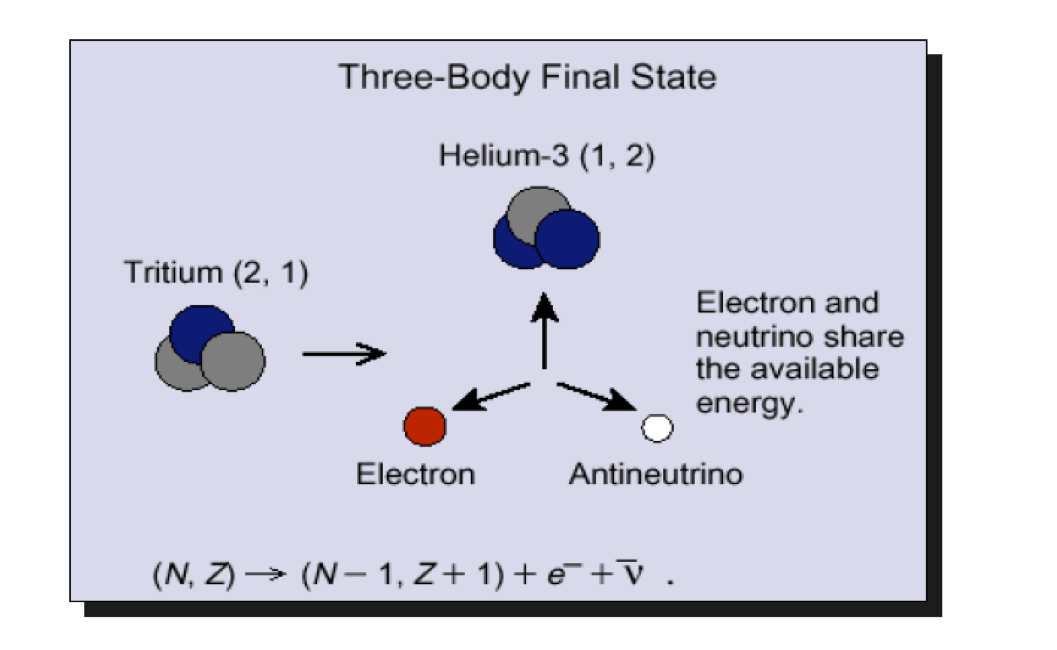
\includegraphics[scale=0.4]{pauli-neutrino.png}
% 
% \column{0.3\textwidth}
%\begin{block}{}
%{\bf Electrically neutral particles which have spin 1/2 and obey the exclusion principle... the mass should be of the order of the electron mass}. 
%\end{block}
%\end{columns}
%\end{frame}

%\begin{frame}
%\frametitle{I have done a terrible thing}
%
%\begin{columns}
%\column{0.35\textwidth}
%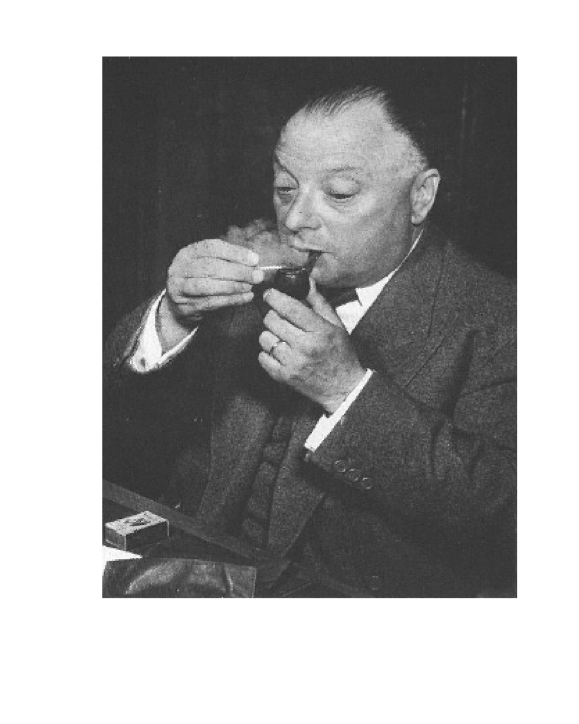
\includegraphics[scale=0.3]{pauli.png}
% 
% \column{0.4\textwidth}
%\begin{block}{}
%Pauli neutral particles had to interact very weakly in order to escape undetected. Furthermore the mechanism by which the ``neutron" was produced was unspecified.
%
%\vspace{0.5cm}
%
%Pauli was unhappy with his brainchild. We wrote: ``I have  done a terrible thing. I have proposed a particle that cannot be detected. It is something no theorist should ever do". 
%
%\end{block}
%\end{columns}
%\end{frame}

%\begin{frame}
%\frametitle{I do not believe in neutrinos}
%\begin{columns}
%\column{0.35\textwidth}
%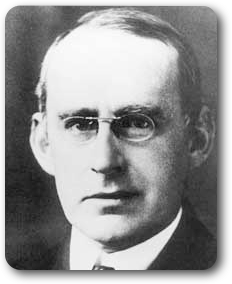
\includegraphics[scale=0.3]{eddington.png}
% 
% \column{0.6\textwidth}
%%\begin{block}{}
%Sir Arthur Eddington: ``Just now nuclear physicists are writing a great deal about hypothetical particles called neutrinos supposed to account for certain peculiar facts observed in $\beta$-ray disintegration. We can perhaps best describe the neutrinos as little bits of spin-energy that have got detached. I am not much impressed by the neutrino theory. In an ordinary way I might say that I do not believe in neutrinos... But I have to reflect that a physicist may be an artist, and you never know where you are with artists. My old-fashioned kind of disbelief in neutrinos is scarcely enough. Dare I say that experimental physicists will not have sufficient ingenuity to make neutrinos?"
%
%%\end{block}
%\end{columns}
%\end{frame}

%\begin{frame}
%\frametitle{The neutron becomes the neutrino}
%\begin{columns}
%\column{0.35\textwidth}
%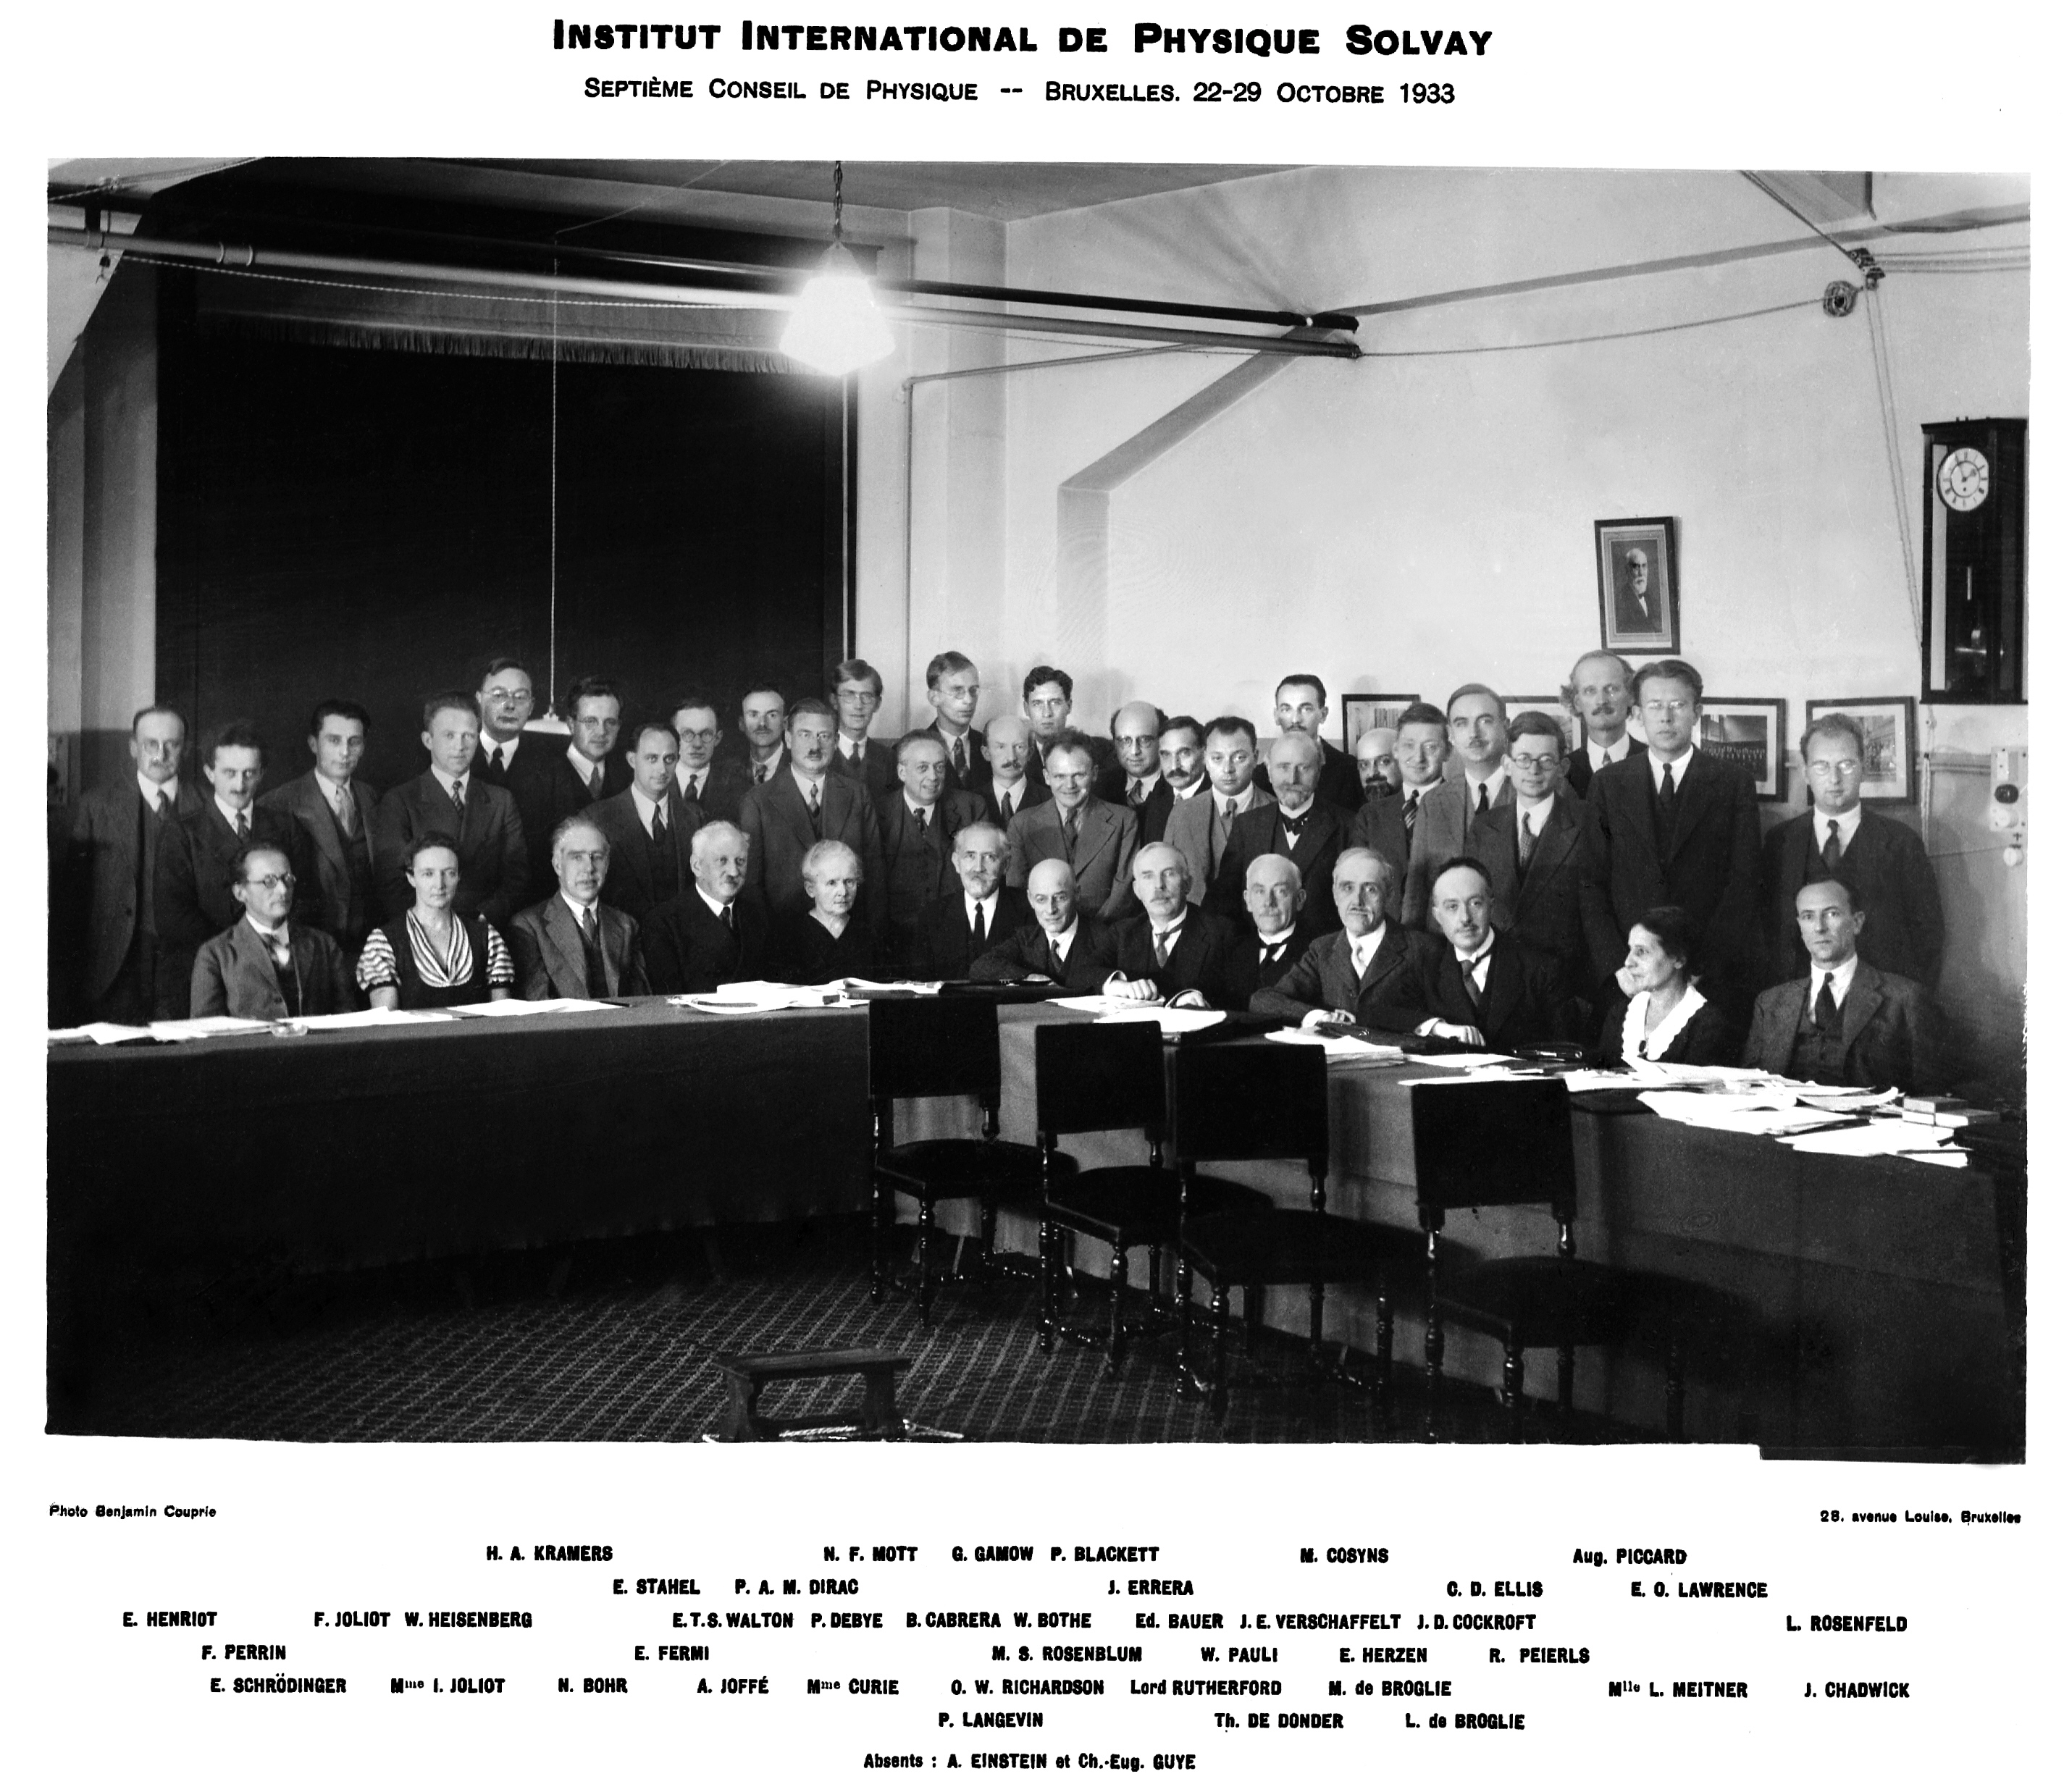
\includegraphics[scale=0.18]{Solvay1933Large.jpg}
% 
% \column{0.6\textwidth}
%%\begin{block}{}
%Pauli in  1933 at the Solvay Congress: ``Regarding the properties of these neutral particles, the atomic weights
%of the radioactive elements tell us first of all that their mass cannot exceed
%much that of the electron. In order to distinguish them from the heavy
%neutrons, Mr. Fermi proposed the name ``neutrino.'' {\bf It's possible that the
%neutrinos' own mass might be equal to zero, so that they would have to
%propagate with the speed of light, like the photons}. However, their penetrating power would exceed by far that of photons of the same energy. It
%seems to me acceptable that the neutrinos have spin 1/2 and satisfy Fermi's 
%statistics, although experiments do not give us any direct proof of this hypothesis. 
%{\bf We know nothing about the interaction of the neutrinos with other material particles and with the photons".}
%
%%\end{block}
%\end{columns}
%\end{frame}